\documentclass[border=4pt]{standalone}

\usepackage{pgfplots}
\usepackage{pgfplotstable}
\usepgfplotslibrary{groupplots}
\usetikzlibrary{patterns}
\pgfplotsset{compat=1.18, width=8.5cm, height=5.6cm, tick label style={font=\small}, label style={font=\small}, legend cell align=left, legend style={font=\small, draw=none, fill=none}}

\definecolor{plnavy}{HTML}{1F4E89}
\definecolor{plrose}{HTML}{B85A52}
\definecolor{plsage}{HTML}{93CC9E}
\definecolor{plsand}{HTML}{E0BE78}
\definecolor{plplum}{HTML}{8E7BB5}
\definecolor{plgray}{HTML}{6E6E6E}

% ==== data: \stackbar{position}{lower share}{middle share}{color}; the top segment fills up to 1 ====
\newcommand{\panelA}{
  \stackbar{1}{0.268}{0.04}{plsage!15}{0.268}
  \stackbar{2}{0.276}{0.03}{plsage!35}{0.276}
  \stackbar{3}{0.244}{0.04}{plsage!55}{0.244}
  \stackbar{4}{0.312}{0.04}{plrose!30}{0.312}
  \stackbar{5}{0.140}{0.07}{plrose!60}{0.140}
  \stackbar{6}{0.169}{0.05}{plsand!25}{0.169}
  \stackbar{7}{0.095}{0.07}{plnavy!65}{0.095}
}
\newcommand{\panelB}{
  \stackbar{1}{0.180}{0.05}{plsage!15}{0.180}
  \stackbar{2}{0.308}{0.04}{plsage!35}{0.308}
  \stackbar{3}{0.232}{0.03}{plsage!55}{0.232}
  \stackbar{4}{0.324}{0.03}{plrose!30}{0.324}
  \stackbar{5}{0.137}{0.06}{plrose!60}{0.137}
  \stackbar{6}{0.157}{0.03}{plsand!25}{0.157}
  \stackbar{7}{0.159}{0.06}{plnavy!65}{0.159}
}
\pgfplotsset{method names/.style={xtick={1,...,7}, xticklabels={A,B,C,D,E,F,Ours}}}
\newcommand{\titleA}{Condition 1}
\newcommand{\titleB}{Condition 2}

\newcommand{\stackbar}[5]{
  \draw[fill=#4, postaction={pattern=north east lines, pattern color=black!75}] (axis cs:#1-0.38,0) rectangle (axis cs:#1+0.38,#2);
  \draw[fill=#4] (axis cs:#1-0.38,#2) rectangle (axis cs:#1+0.38,{#2+#3});
  \draw[fill=#4] (axis cs:#1-0.38,{#2+#3}) rectangle (axis cs:#1+0.38,0.9);
  \draw[fill=#4, postaction={pattern=crosshatch, pattern color=black!75}] (axis cs:#1-0.38,0.9) rectangle (axis cs:#1+0.38,1);
  \node[font=\tiny, fill=white, inner sep=1pt, rounded corners=1pt] at (axis cs:#1,{#2/2}) {#5};
}

\begin{document}
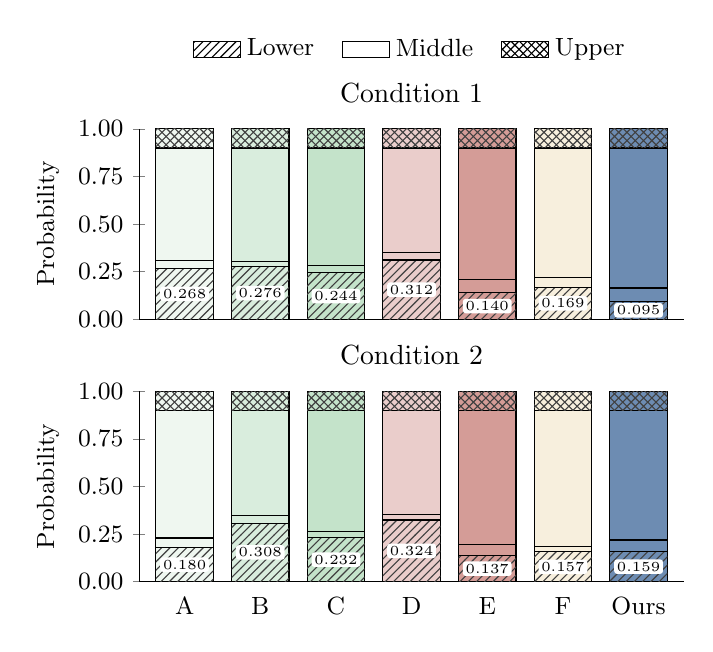
\begin{tikzpicture}
\begin{groupplot}[group style={group size=1 by 2, vertical sep=26pt, x descriptions at=edge bottom}, width=8.5cm, height=4cm, ymin=0, ymax=1, xmin=0.4, xmax=7.6, axis lines=left, axis line style={-}, xtick style={draw=none}, ytick={0,0.25,0.5,0.75,1}, ylabel={Probability}, method names, yticklabel style={/pgf/number format/fixed, /pgf/number format/precision=2, /pgf/number format/fixed zerofill}]
  \nextgroupplot[title={\titleA}, legend style={at={(0.5,1.3)}, anchor=south, legend columns=3, /tikz/every even column/.append style={column sep=8pt}}]
    \addlegendimage{area legend, draw=black, pattern=north east lines}\addlegendentry{Lower}
    \addlegendimage{area legend, draw=black, fill=white}\addlegendentry{Middle}
    \addlegendimage{area legend, draw=black, pattern=crosshatch}\addlegendentry{Upper}
    \panelA
  \nextgroupplot[title={\titleB}]
    \panelB
\end{groupplot}
\end{tikzpicture}
\end{document}
